% !TEX root = ../build-polygon/proof-recursion.tex

\subsection{Recursion}

\subsubsection{Setup Phase}

Since verifiers are much more efficient than provers, we can use this fact to create a recursive cascade of verifiers in which at each step we achieve a proof that can be more efficiently verified.
In our architecture, we create a chain of STARK verifiers using intermediate circuits for the definition of these STARK verifiers as shown in Figure \ref{fig:recursion-setup}.
We use circuits because they are suitable for computations with limited branching and a verifier is a computation of this type.

\begin{figure}[H]
\centering
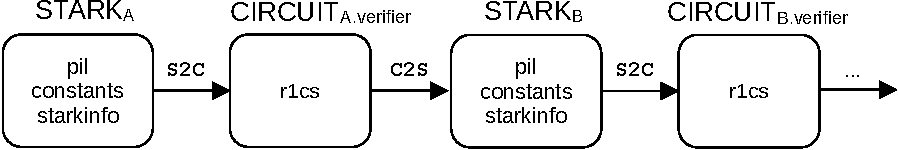
\includegraphics[width=0.8\textwidth]{\recursiondir/figures/recursion-setup}
\caption{Recursion setup.}
\label{fig:recursion-setup}
\end{figure}

Following Figure \ref{fig:recursion-setup}, lets consider that 
we have the parameters that describe the first STARK (pil, constants and starkinfo).
This first STARK that we denote as $\texttt{STARK}_{\texttt{A}}$, is then automatically translated into its verifier circuit. 
The STARK verifier circuit is described with R1CS constraints.
This translation, that we call \stoc (STARK-to-CIRCUIT), is performed in a setup phase. In other words, the R1CS description of the STARK verifier circuit can be pre-processed before the computation of the proof. 
We use Circom as intermediate representation language for the description of the circuits (see Section \ref{subsec:stoc} for more details about \stoc).

Next, we take the circuit definition (R1CS) and automatically translate it into a new STARK definition, that is to say, a new pil, new constants and a starkinfo.
This translation, that we call \ctos (CIRCUIT-to-STARK), 
is performed also in a setup phase.
Following our example, the new generated STARK is denoted as
$\texttt{STARK}_{\texttt{B}}$ and it is essentially a \plonk{ish} arithmetization with some custom gates of the verification circuit of $\texttt{STARK}_{\texttt{A}}$
(for more details about \stoc see Section \ref{subsec:ctos}).
It is worth to mention that these recursion steps can be applied as many times as desired taking into account that each step will compress the proof making it
more efficient to verify but increasing the prover complexity.
Finally, remark that during the setup phase, several artifacts for generating each STARK prover are generated (see Sections \ref{subsec:stoc} and \ref{subsec:ctos} for more information 
about these artifacts). 

\subsubsection{Proving Phase \label{subsubsec:proving:phase:intro}}


The first proof is generated by providing the proper inputs and public values to the first STARK prover. Then, the output proof is passed as input to the next STARK prover together with the public inputs and the process is recursively repeated.
In Figure \ref{fig:recursive-provers} we show how in essence a chain of recursive STARK provers work.

\begin{figure}[H]
\centering
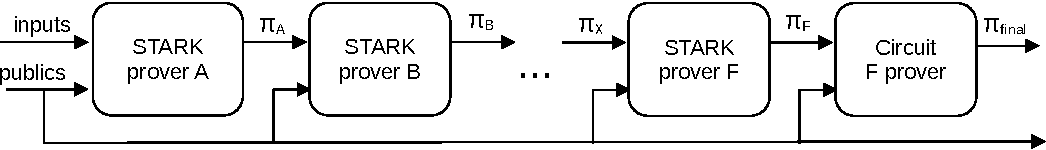
\includegraphics[width=0.95\textwidth]{\recursiondir/figures/recursive-provers}
\caption{Recursive provers.}
\label{fig:recursive-provers}
\end{figure}

Notice that the final proof is actually a circuit-based proof (currently we are using a Groth16 proof). More details about the proving phase can be found in Section \ref{subsec:recursion:step:proof}.


\subsection{Aggregation} 

Our architecture also allows aggregation when generating the proofs. Aggregation is a particular type of proof composition in which multiple valid proofs can be all proven to be valid by comprising them all into one proof, called the \textit{aggregated proof}, and only validating the aggregated one.
In our architecture, aggregators are defined in intermediate circuits.
Figure \ref{fig:aggregation_example} shows an example of aggregation with binary aggregators.
\begin{figure}[H]
\centering
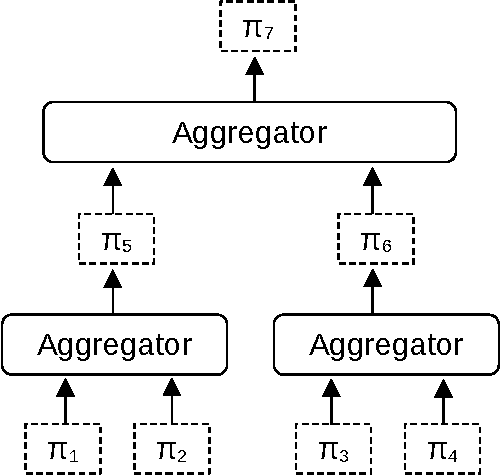
\includegraphics[width=0.4\textwidth]{\recursiondir/figures/radix-2-aggregation}
\caption{Aggregation example.}
\label{fig:aggregation_example}
\end{figure}


\subsection{Setup \stoc \label{subsec:stoc}}

Recall that we denote \stoc to the process of converting a given STARK into its verifier circuit, which is described in Circom and compiled to the corresponding R1CS constraints. The architecture of this generic conversion is depicted in Figure \ref{fig:setup-p2c}, where a \texttt{STARK}$_\texttt{x}$ is converted into a circuit denoted as $C_y$.


\begin{figure}[H]
\centering
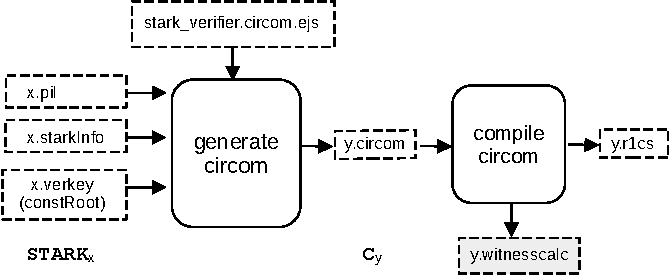
\includegraphics[width=0.8\textwidth]{\recursiondir/figures/setup-s2c}
\caption{Setup \stoc.}
\label{fig:setup-p2c}
\end{figure}

The input of the \stoc step is all the information needed to set up a circuit verifying the given STARK. 
In our architecture this is a PIL file specifying the STARK constraints that are going to be validated and the polynomial names, a \texttt{starkInfo} file containing the FRI-related parameters (blowup factor, the number of queries to be done, etc.), 
and the Merkle tree root of the computation constants (\texttt{constRoot}).
The output of the generate Circom process is a Circom description. 
The circuit is actually generated by filling an  \texttt{EJS} template
for the Circom description using the constraints defined by the PIL, the FRI-related parameters included by the \texttt{starkInfo} file and the \texttt{constRoot}. 
As shown in Figure \ref{fig:stark-verifier-circuit}, the inputs of the generated STARK verifier circuits are divided in two groups: the public inputs and the private inputs.

\begin{figure}[H]
\centering
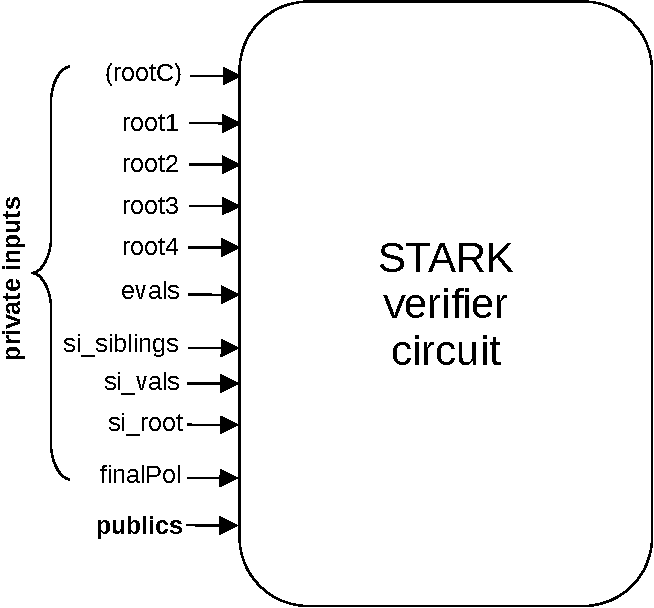
\includegraphics[width=0.55\textwidth]{\recursiondir/figures/STARK-verifier-inputs}
\caption{Inputs of the STARK verifier circuits.}
\label{fig:stark-verifier-circuit}
\end{figure}

The private inputs are the parameters of the previous STARK proof:

%TODO: Marc -> All: Enable should be reviewed
%TODO: Jose -> All: review description with info from Roger

\begin{itemize}

\item \texttt{(rootC)}: Four field elements being the root of the Merkle tree for the evaluations of constant (that is, preprocessed) polynomials of the previous STARK.
In some of the intermediate circuits that we generate, \texttt{rootC} is an input of the circuit while in other generated circuits \texttt{rootC} are internal signals 
hardcoded to the corresponding values (more information for each particular case is provided later).

\item \texttt{root1}: Four field elements being the root of the Merkle tree for the evaluations of all the trace column polynomials for the execution trace. 

\item \texttt{root2}: Four field elements being the root of the Merkle tree for the evaluations of the $h$ polynomials appearing in each lookup argument of the previous STARK. This root may be $0$ if no lookup argument is provided in the PIL.  

\item \texttt{root3}: Four field elements being the root of the Merkle tree for the evaluations of the grand product polynomials appearing in each argument (that is, lookup, permutation or connection arguments) of the previous STARK and the intermediate polynomials appearing in certain splitting of them. This root may be $0$ if no arguments are provided in the PIL. 

\item \texttt{root4}: Four field elements being the root of the Merkle tree for the evaluations of the splitting $Q_1$ and $Q_2$ of the $Q$ polynomial of the previous STARK.

\item \texttt{evals}: Contains all the necessary evaluations for all the polynomials appearing in the FRI verification process at a challenge value $z$ and at $gz$. 

\item \texttt{si\_root}: Four field elements being their root of the Merkle tree for the evaluations of the $i$-folded FRI polynomial, that is, the polynomial appearing in the $i$-th step of the FRI verification. 

\item \texttt{si\_vals}: The leaves' values of the previous Merkle tree used to check all the queries. The total amount of such values depends on the number of queries and the reduction factor attached to the current step of the FRI. 


\item \texttt{si\_siblings}: Merkle proofs for each of the previous evaluations.

\item \texttt{finalPol}: Contains all the evaluations of the last step's folding polynomial constructed in the FRI verification procedure over the last defined domain which has the same size as the degree of the polynomial. 

\end{itemize}

The \texttt{publics} are a set of inputs that will be used by the verifier to check the final prove and also by the intermediate STARKs (more information about publics used in the zkEVM STARK is provided in Section \ref{subsec:zkEVM:architecture}).

The final process to complete the \stoc step is to compile the Circom description to obtain a file with the associated R1CS constraints and a witness calculator program capable of compute all the values of the circuit wires for a given set of inputs.

Finally, remark that the particular intermediate circuit generated in a \stoc step,  denoted as $C_y$ in Figure \ref{fig:setup-p2c}, can be just a verifier of the previous STARK (\texttt{STARK}$_\texttt{x}$ in Figure \ref{fig:setup-p2c}) if we are only applying a recursion step, but more generally, other types of circuits that include the verifier but provide more functionality can be used. 
This latter is the case when we use circuits to verify aggregation of proofs.


\subsection{Setup \ctos \label{subsec:ctos}}

In our proving architecture, we create a chain of STARKs. 
From the \stoc step we can obtain a circuit that has to be converted again 
into a STARK. 
The step that achieves this conversion is a pre-processing step 
that we call \ctos. A picture of a generic \ctos step can be found in Figure \ref{fig:setup-c2s}, where a circuit denoted as $C_y$
is converted into its corresponding STARK (\texttt{STARK}$_\texttt{y}$).

\begin{figure}[H]
\centering
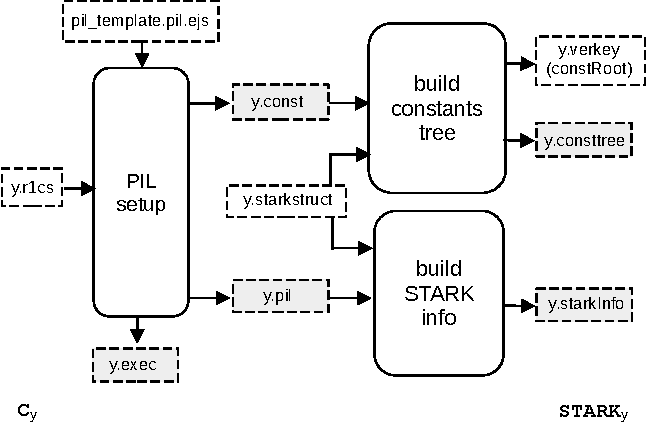
\includegraphics[width=0.75\textwidth]{\recursiondir/figures/setup-c2s}
\caption{Setup recursion step \ctos.}
\label{fig:setup-c2s}
\end{figure}

In more detail, the STARK arithmetization of the intermediate circuits of our proving architecture is a \plonk{ish} arithmetization with custom gates and using 12 polynomials for the values of the gate wires of the computation trace. The STARK arithmetization includes several custom gates for doing specific tasks more efficiently. In particular, the custom gates provide the following functionality:

\begin{itemize}
\item \textbf{Poseidon}: This custom gate is capable of validating a Poseidon hash from a given $8$ field elements as inputs, $4$ field elements as capacity and a variable number of output elements. More specifically, this circuit implements the MDS matrix and the $7$-th power of field elements computations used to execute each of the rounds defined by the Poseidon hash sponge construction. 
\item \textbf{Extended Field Operations}: This custom gate is capable of validating multiplications and additions (or a combination of both) over the extended field $\FF_{p^3}$. The inputs are $3$ elements $a, b, c \in \FF_{p^3}$ and the output is corresponds to the element 
\[
a \cdot b + c \in \FF_{p^3}
\]
where the operations are defined over $\FF_{p^3}$. Observe that defining $c$ equal to $0$ one can compute pure multiplications. Similarly, setting $b$ equal to $1$, pure additions can be computed. 

\item \textbf{FFT}: This custom gate is in charge of computing FFT of a variable size in $\FF_p$ or in an extension field. 

\item \textbf{Polynomial Evaluation}: This custom gate is in charge of computing a single evaluation of polynomials in $\FF_{p^3}$ using Horner's rule. The input consists on a field element $z \in \FF_{p^3}$ and the coefficients of the polynomial $p$ which we are going to evaluate. The output is the evaluation $p(z) \in \FF_{p^3}$. 
\end{itemize}

We use selector polynomials to activate the custom gates of our STARK. 
These polynomials are constant (pre-processed). In particular, we use the selectors \texttt{POSEIDON12}, \texttt{GATE}, \texttt{CMULADD}, \texttt{EVPOL4} and \texttt{FFT4} are introduced. The selector \texttt{GATE} is actually in charge of activating a basic \plonk gate. The other selectors are in charge of selecting whichever subcircuit needs to be executed. Moreover, there also exist a special selector called \texttt{PARTIAL} which is in charge of distinguishing between partial and full layers in the Poseidon, since this affects the relationships between the values.

At this point we can detail the processes of the \ctos step.
As shown in Figure \ref{fig:setup-c2s}, the first process of the \ctos step is the PIL setup, which takes the R1CS constraints of a given intermediate circuit as input and produces all the STARK-related artifacts.
This includes the associated STARK identity constraints and the computation constants
that are respectively stored in a PIL file (\texttt{y.pil}) and in a file of constants
(\texttt{y.const}).
In particular, the identity constraints of the \plonk{ish} arithmetization are generated by filling an \texttt{EJS} template for the associated PIL (for the zkEVM the template used is called \texttt{compressor12.pil.ejs}). For a complete description of the the \texttt{c12} arithmetization refer to Section \ref{sec:c12}.

The PIL setup also generates an important file with exec extension (\texttt{y.exec})
that defines how to rearrange the values produced by the circuit witness calculator into the appropriate values of the STARK execution trace (see Thaler's book for more information about this rearrangement process). 
Notice that the rearrangement rules and the computation constants only depend on 
the circuit shape (which is coded in the \texttt{.r1cs} file generated by the Circom compiler). In other words, these parameters do not depend on the particular values of the circuit wires computed for a particular input.
Nevertheless, we will use the rearrangement rules file together with the witness values for a given input later on to build the STARK execution trace, which in turn is needed to generate the STARK proof.

Finally, we also produce the \texttt{starkInfo} file and a Merkle tree with the STARK constants.

\subsection{Recursion Step Proof \label{subsec:recursion:step:proof}}

As we explained in Section \ref{subsubsec:proving:phase:intro}, to generate the final proof, we have to compute the proof of each 
intermediate STARK (see Figure \ref{fig:recursive-provers}).
Each intermediate STARK proof is generated using the witness values provided by the execution of the associated circuit witness computation program using as inputs the publics and the values of the previous proof.
Then, these values are properly rearranged to build the STARK execution trace using the corresponding \texttt{.exec} file.
In Figure \ref{fig:recursion:step:proof}, we provide the scheme of how the proof of an intermediate STARK is generated. 

\begin{figure}[H]
\centering
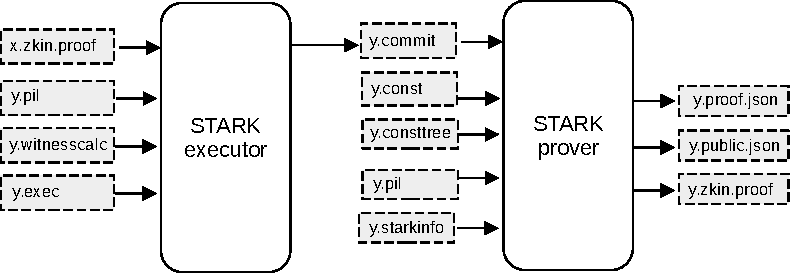
\includegraphics[width=0.9\textwidth]{\recursiondir/figures/recursive-step-proof}
\caption{STARK \texttt{Proof} of a recursion step.}
\label{fig:recursion:step:proof}
\end{figure}

As it can be observed, the STARK executor process takes the parameters of previous proof and the public inputs (both in the file \texttt{x.zkin.proof} which
has the proper format for the witness calculator generated by the Circom compiler), the PIL of the current STARK (\texttt{y.pil}), the witness calculator program of the associated circuit (\texttt{y.witnesscalc}) and the file of rearrangement rules (\texttt{y.exec}) to generate the non-preprocessed part of the STARK execution trace (\texttt{y.commit}). 
Next, the STARK prover process takes the execution trace, that is to say, the committed and constant polynomials, the constant tree, the corresponding PIL file and the information provided by the \texttt{zkevm.starkinfo.json} file to generate the proof.
Finally, when the proof is generated, the STARK prover process generates three files:

\vspace{0.1cm}
\begin{compactitem}
\item \textbf{Proof File} (\texttt{y.proof.json}): A json file containing the whole STARK proof in a \texttt{.json} file. 

\item \textbf{Publics File} (\texttt{y.public.json}): A json file containing only the publics. 

\item \textbf{zkIn File} (\texttt{y.zkin.proof.json}): A json file combining both the proof and the publics. 
\end{compactitem}